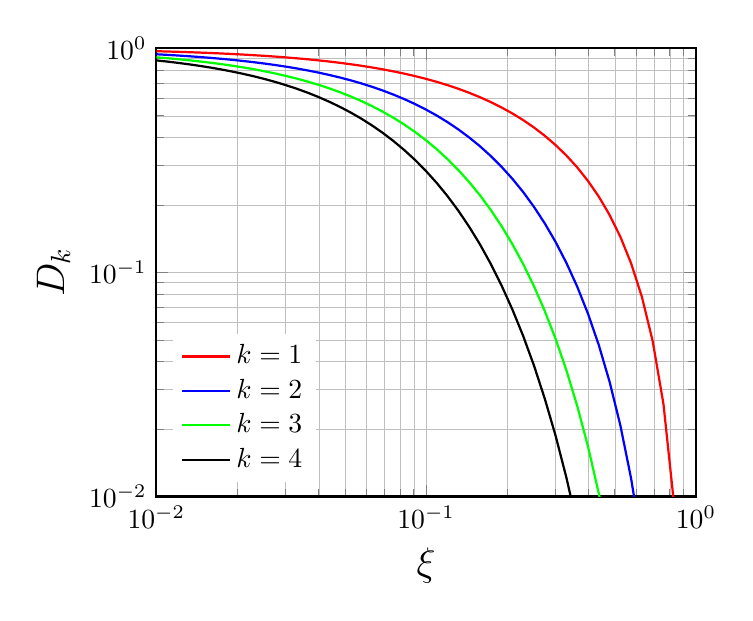
\begin{tikzpicture}
    \pgfmathsetmacro{\pi}{3.141592653589793}     % dépassement d4 
    \begin{axis}[
            xmode=log,
            ymode=log,
        legend style={draw=none},
        legend pos=south west,
        axis line style = thick,
        xmin=0.01,
        xmax=1,
        ymin=0.01,
        ymax=1.0,
        xlabel={$\xi$},
        ylabel={$D_k$},
        label style={font=\Large},
        grid=both,
        grid style={line width=.1pt, draw=gray!50},
        major grid style={line width=.2pt,draw=gray!50},
        ]
        \addplot[thick,color=red,domain=0.0001:1, samples=101]{exp(-(x*\pi)/(sqrt(1-x*x)))};
        \addplot[thick,color=blue,domain=0.0001:1, samples=101]{exp(-(2*x*\pi)/(sqrt(1-x*x)))};
        \addplot[thick,color=green,domain=0.0001:1, samples=101]{exp(-(3*x*\pi)/(sqrt(1-x*x)))};
        \addplot[thick,color=black,domain=0.0001:1, samples=101]{exp(-(4*x*\pi)/(sqrt(1-x*x)))};
        \legend{$k=1$,$k=2$,$k=3$,$k=4$}
    \end{axis}
\end{tikzpicture}

